\documentclass[12pt,fleqn]{article}\usepackage{../common}

\begin{document}
Google Nasil Isler? 

Google arama motoruna bir kelime yazdigimizda geri gelen sonuclar nasil
kararlastirilir? Ilk akla gelen yontem tabii ki Web'deki tum sayfalarin
(milyarlarca sayfa) sayfalar uzerindeki kelimelerin o sayfa ile
iliskilendirilmesi ve arama yapilinca kelimeye gore sayfa geri
getirilmesi. Mesela alttaki ornekte ``book (kitap)'' yazinca geriye 1.,
2. ve 5. sayfalar geri gelecek. Fakat hangi sirada? Bu sayfalardan hangisi
digerlerinden daha onemli?

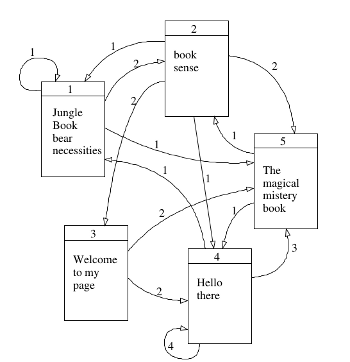
\includegraphics[height=9cm]{pg2.png}

Google'in arama motorlarina getirdigi en buyuk yeniliklerden biri PageRank
algoritmasidir. Bu algoritmanin temelinde daha fazla referans edilen
sayfalar daha ustte cikmasi yatar. Hatta o referans eden sayfalarin
kendilerine daha fazla referans var ise bu etki ta en sondaki sayfaya kadar
yansitilir, hatta bu zincir bastan sona her seviyede hesaplanabilir. Peki bu
nasil gerceklestirilir?

PageRank Web sayfalarini bir Markov Zincir olarak gorur. Markov Zincirleri
seri halindeki $X_n, n=0,1,2,..$ rasgele degiskenini modeller ve bu
degiskenler belli sayidaki konumlarin birinde olabilirler. Mesela konumlari
bir dogal sayi ile ilintilendirirsek $X_n = i$ olabilir ki $i=\{0,1,..\}$
diye kabul edelim. 

Markov Zincirlerinde (MZ) $i$ konumundan $j$ konumuna gecis olasiligini,
$P_{ij}$, biliriz ve bu $P(X_{n+1} = j | X_{n} = i)$ olarak acilabilir. Acilimdan  
gorulecegi uzere bir MZ sonraki adima gecis olasiligi icin sadece
bir onceki adima bakar. Bu tur once/sonra yapisindaki iki boyutlu hal, 
cok rahat bir sekilde matrisina cevirilebilir / gosterilebilir. Onceki konum 
satirlar, sonraki konum kolonlar olarak betimlenir mesela. 

Ornek

Bir sonraki gunde yagmur yagmayacagini bir MZ olarak tasarlayalim. Bir
sonraki gunde yagmur yagmayacagini sadece bugun etkiliyor olsun. Eger bugun
yagmur yagiyorsa yarin yagmur yagmasi 0.7, eger bugun yagmiyor ise yarin
yagmasi 0.4. MZ soyle

$$ 
P =
\left[\begin{array}{cc}
0.7 & 0.3 \\
0.4 & 0.6
\end{array}\right]
 $$

Gecis olasiliklarindan bahsettigimize gore ve elimizde sinirli / belli
sayida konum var ise, bir MZ'nin her satirindaki olasiliklarin toplami
tabii ki 1'e esit olmalidir. 

MZ'lerin ilginc bir ozelligi $n$ adim sonra $i,j$ gecisinin $P^n$ hesabiyla
yapilabilmesidir. Yani $P$'yi $n$ defa kendisiyle carpip $i,j$ kordinatina 
bakarsak $n$ adim sonrasini rahatca gorebiliriz. Bunun ispatini burada
vermeyecegiz. 

Mesela ustteki ornekte, eger bugun yagmur yagiyorsa 4 gun sonra yagmur
yagma olasiligi nedir? 

\begin{minted}{python}
import numpy.linalg as lin
P = np.array([[0.7,0.3],[0.4,0.6]])
P4 = lin.matrix_power(P,4)
print P4
\end{minted}

\begin{verbatim}
[[ 0.5749  0.4251]
 [ 0.5668  0.4332]]
\end{verbatim}

Aradigimiz gecis icin kordinat 0,0'a bakiyoruz ve sonuc 0.5749. Numpy
\verb!matrix_power! bir matrisi istedigimiz kadar kendisiyle carpmamizi
sagliyor. 

Duragan Dagilim (Stationary Distribution)

Eger yagmur ornegindeki matrisi carpmaya devam edersek, mesela 8 kere
kendisiyle carpsak sonuc ne olurdu? 

\begin{minted}{python}
import numpy.linalg as lin
P = np.array([[0.7,0.3],[0.4,0.6]])
P8 = lin.matrix_power(P,8)
print P8
\end{minted}

\begin{verbatim}
[[ 0.57145669  0.42854331]
 [ 0.57139108  0.42860892]]
\end{verbatim}

Dikkat edilirse, her satir bir deger yaklasmaya basladi. Bu deger MZ'nin
duragan dagilimidir, belli kosullara uyan her MZ'nin boyle bir duragan
dagilimi vardir. Bu kosullar MZ'nin periyodik olmayan (aperiodic) ve tekrar
eden (recurrent) olmasidir. Bu sartlar cok ``ozel'' sartlar degildir
aslinda, daha cok ``normal'' bir MZ'yi tarif ediyor diyebiliriz. Tum
konumlari tekrar eden yapmak kolaydir, MZ tek bagli (singly connected) hale
getirilir, yani her konumdan her diger konuma bir gecis olur, ve periyodik
olmamasi icin ise MZ'ye olmadigi zamanlarda bir konumdan kendisine gecis
saglanir (az bir gurultu uzerinden). 

Nihayetinde duraganlik su denkleme sebebiyet verir, 

$$ \pi = \pi P $$

Burada duragan dagilim $\pi$'dir. Bu denklem tanidik geliyor mu?  Devrigini
alarak soyle gosterelim, belki daha iyi taninir, 

$$ P^T\pi^T = \pi^T $$

Bir sey daha ekleyelim, 

$$ P^T\pi^T = 1 \cdot \pi^T $$

Bu ozdeger/vektor formuna benzemiyor mu? Evet! Bu form 

$$ Ax = \lambda x $$

MZ denklemi sunu soyluyor, 1 degerindeki ozdegere ait ozvektor bir MZ'nin
duragan dagilimidir! Bu arada, MZ gecis matrisi $P$'nin en buyuk
ozdegerinin her zaman 1 oldugunu biliyoruz. Bu durumda en buyuk ozdegere
ait ozvektoru hesaplamak yeterli olacaktir. Bunu yapmayi zaten {\em Lineer
  Cebir Ders 21}'de ogrenmistik, ust metot (power method) sayesinde bu
hesap kolayca yapilabiliyor.

Simdi en basktaki Web sayfalarina ait gecisleri yazalim,

\begin{minted}{python}
P = [[1./4, 2./4, 0, 0, 1./4],
     [1./6, 0, 2./6, 1./6, 2./6],
     [0, 0, 0, 2./4, 2./4],
     [1./8, 0, 0, 4./8, 3./8],
     [0, 1./2, 0, 1./2, 0]]

P = np.array(P)
print P
\end{minted}

\begin{verbatim}
[[ 0.25        0.5         0.          0.          0.25      ]
 [ 0.16666667  0.          0.33333333  0.16666667  0.33333333]
 [ 0.          0.          0.          0.5         0.5       ]
 [ 0.125       0.          0.          0.5         0.375     ]
 [ 0.          0.5         0.          0.5         0.        ]]
\end{verbatim}

Simdi ust metotu kullanarak duragan dagilimi hesaplayalim. Herhangi bir
baslangic vektorunu $P$ ile 20 kere  carpmak yeterli olur.

\begin{minted}{python}
import numpy.linalg as lin
x=np.array([.5, .3, .1, .1, 0]) # herhangi bir vektor
for i in range(20): 
    x = np.dot(x,P)
print 'pi = ', x
\end{minted}

\begin{verbatim}
pi =  [ 0.10526316  0.18421053  0.06140351  0.38596491  0.2631579 ]
\end{verbatim}

Not: Aslinda cebirsel olarak $P$'yi 20 kere kendisiyle carpmak ve sonucu
baslangic vektoru ile bir kere carpmak ta dusunulebilirdi. Fakat 20 kere
vektor / matris carpimlari yapmak, 20 kere matris / matris carpimi
yapmaktan daha verimli olacaktir. Buyuk Veri ortami icin de bu soylenebilir.

Eger kutuphane cagrisi kullanmak gerekirse, 

\begin{minted}{python}
import numpy.linalg as lin
evals,evec = lin.eig(P.T)
pi =  evec[:,0] / np.sum(evec[:,0])
print np.abs(pi)
\end{minted}

\begin{verbatim}
[ 0.10526316  0.18421053  0.06140351  0.38596491  0.26315789]
\end{verbatim}

Sonuc gosteriyor ki ``book'' yazdigizda Google bize 5. sayfayi en basta
olacak sekilde sonuc dondurmeli, cunku onun duragan dagilimi 1,2,5
sayfalarinin arasinda en yuksek.

Duragan Dagilima Bakis

MZ ve duragan dagilimin PageRank'le alakasini bir daha dusunelim. MZ ile
$n$ adim sonrasini hesaplayabiliyoruz, duragan dagilim ise sonsuz adim
sonrasini ifade ediyor. Ve bu dagilim, bir anlamda, sonsuz yapilan adimlar
sirasinda {\em en fazla hangi konumlarda} zaman gecirilecegini
gosteriyor. Konum yerine sayfa dersek duragan dagilimin niye en onemli
sayfalari belirlemek icin onemli oldugunu anlariz. 

Kullanici herhangi bir sayfada iken hangi diger sayfalara gidecegi o sayfa
uzerinde baglantilar uzerinden anlasilir, PageRank bu baglantinin
mevcudiyetine bakar sadece, o mevcudiyet uzerinden bir gecis olasiligi
hesaplar, ve bu olasiliga gore (raslantisal sekilde) baglantinin takip
edilecegi dusunulur. Bu arada cogunlukla sayfalar arasindaki baglantilarin
agirligi 1 olacaktir, fakat ornek amacli 2,3 gibi sayilar da kullaniliyor. 

Rasgele Sayfa Gecisi

Simdi $\pi^T$ yerine $p$, $P$ yerine $N$ kullanalim, PageRank ozyineli
algoritmasi 

$$ p = N^Tp $$ 

olarak gosterilebilir. Google veri temsili uzerinde bazi ekler yapmaktadir,
mesela kullanicinin hicbir baglanti takip etmeyip tarayiciya direk URL
girerek baska bir sayfaya ziplamasi (teleporting) bir sekilde temsil
edilmelidir. Ayrica hic disa baglanti vermeyen sayfalar (olu noktalar)
hesaba katilmalidir. 

Bu her iki durum icin formul su sekilde ikiye ayirilir,

$$ p = (1-d)N^Tp + dN_f^Tp $$

$$ = ((1-d)N^T + dN_f^T) p $$

$$ = M^Tp $$

ki,

$$M = (1-d)N^T + dN_f^T$$ 

olacaktir. $N_f$ bir normalize edilmis ``ziplama'' matrisidir, yani her
sayfadan her diger sayfaya bir baglanti ``varmis gibi'' yapar, mesela 5x5
boyutunda tum ogeleri 0.20 olacaktir. $d$ bir agirlik sabitidir, Google'in
bunu 0.85 olarak tanimladigi duyulmustur, ve gercek baglanti matrisi ve
rasgele ziplama matrisi arasinda bir agirlik tanimlar, her ikisinde de
birazcik alarak (daha cok ana $N$'den tabii) niahi matrisi olusturur. Ornek
olarak su grafige bakalim, 

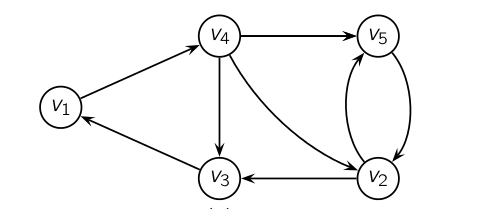
\includegraphics[height=4cm]{pg3.png}

\begin{minted}{python}
N = [[0, 0, 0, 1., 0],
     [0, 0, 1./2, 0, 1./2],
     [1, 0, 0, 0, 0],
     [0, 1./3, 1./3, 0, 1./3],
     [0, 1, 0, 0, 0]]

N = np.array(N)

Nf = 0.20 * np.ones((5,5))
d = 0.85
M = d*N + (1-d)*Nf
x=np.array([.5, .3, .1, .1, 0]) # herhangi bir vektor
for i in range(20): 
    x = np.dot(x,M)
print 'result = ', x 
\end{minted}

\begin{verbatim}
result =  [ 0.18959094  0.24375097  0.18775335  0.19115138  0.18775335]
\end{verbatim}

Sonuca gore $v_2$ en yuksek PageRank degerine sahip. 

[1] Murphy, K., CS340: Machine Learning Lecture Notes, \url{www.ugrad.cs.ubc.ca/~cs340}

[2] Ross, S., Introduction to Probability Models, 8th Edition

[3] Zaki, Maira, Fundamentals of Data Mining Algorithms

\end{document}
